\chapter{Lec 03 - PCA}

\section{Unsupervised Learning}
Most of this course focuses on \textbf{supervised learning} methods such as regression and classification. In that setting we observe both a set of features $X_1, X_2, . . . , X_p$ for each object, as well as a response or
outcome variable $Y$. The goal is then to predict $Y$ using $X_1, X_2, . . . , X_p$.\\\\
Here we instead focus on \textbf{unsupervised learning}, where we observe only the features $X_1, X_2, . . . , X_p$. We are not interested in prediction, because we do not have an associated response variable $Y$. The goal is to discover interesting things about the measurements: is there an informative way to visualize the data? Can we discover subgroups among the variables or among the observations?

\section{Recall of mean, variance, covariance}
Recall of the formulas for mean, variance and covariance:
\begin{itemize}
    \item \textbf{Mean:} $\overline{X} = \frac{1}{n}\sum_{i=1}^n x_i$

    \item \textbf{Variance:} $Var(X) = \frac{1}{n}\sum_{i=1}^n (x_i - \overline{X})^2$

    \item \textbf{Covariance:} $Cov(X,Y) = \frac{1}{n}\sum_{i=1}^n (x_i - \overline{X})(y_i - \overline{Y})$
\end{itemize}

\section{Principal Components Analysis (PCA)}
PCA produces a low-dimensional representation of a dataset. It finds a sequence of linear combinations of the variables that have maximal variance, and are mutually uncorrelated.
\\\\
PCA is an unsupervised approach, since it involves only a set of features $X_1, X_2,...,X_p$, and no associated response $Y$. Apart from producing derived variables for use in supervised learning problems, PCA also serves as a tool for data visualization.

\subsection{What Are Principal Components?}
Suppose that we wish to visualize $n$ observations with measurements on a
set of $p$ features, $X_1, X_2,...,X_p$, as part of an exploratory data analysis. We would like to find a low-dimensional representation of the data that captures as much of the information as possible. For instance, if we can obtain a two-dimensional representation of the data that captures most of the information, then we can plot the observations in this low-dimensional space.\\\\
PCA provides a tool to do just this. It finds a low-dimensional representation of a data set that contains as much as possible of the variation. The idea is that each of the $n$ observations lives in $p$-dimensional space, but not all of these dimensions are equally interesting. PCA seeks a small number of dimensions that are as interesting as possible, where the concept of interesting is measured by the amount that the observations vary along each dimension.  Each of the dimensions found by PCA is a linear combination of the $p$ features. We now explain the manner in which these dimensions, or principal components, are found.\\\\
The \textit{first principal component} of a set of features $X_1, X_2,...,X_p$ is the normalized linear combination of the features
\[Z_1 = \phi_{11}X_1 + \phi_{21}X_2 + ... +\phi_{p1}X_p\]
that has the largest variance. By normalized, we mean that $\sum_{j=1}^p \phi_{j1}^2 = 1$. We refer to the elements $\phi_{11},...,\phi_{p1}$ as the loadings of the first principal component; together, the loadings make up the principal component loading vector $\phi_1$. We constrain the loadings so that their sum of squares is equal to one, since otherwise setting these elements to be arbitrarily large in absolute value could result in an arbitrarily large variance.\\\\
Given a $n \times p$ data set $\textbf{X}$, how do we compute the first principal component? Since we are only interested in variance, we assume that each of the variables in $\textbf{X}$ has been centered to have mean zero (that is, the column means of $\textbf{X}$ are zero) \footnote{We can do this by subtracting the mean of each column from the values of that column.}. We then look for the linear combination of the sample feature values of the form:
\begin{equation}
    z_{i1} = \phi_{11}x_{i1} + \phi_{21}x_{i2} + ... +\phi_{p1}x_{ip}
    \label{z}
\end{equation}
that has \textbf{largest sample variance}, subject to the constraint that $\sum_{j=1}^p \phi_{j1}^2 = 1$. In other words, the first principal component loading vector solves the optimization problem:
\begin{equation}
    \text{maximize}_{\phi_{11}, ..., \phi_{p1}}\left\{\frac{1}{n}\sum_{i=1}^n\left(\sum_{j=1}^p \phi_{j1}x_{ij}\right)^2\right\} \quad \text{subject to } \sum_{j=1}^p \phi_{j1}^2 = 1
    \label{first comp}
\end{equation}
From \ref{z}, we can write the objective in \ref{first comp} as:
\[\frac{1}{n}\sum_{i=1}^n z_{i1}^2\]
Note that in \ref{first comp} the variance is computed without subtracting the mean because, since $\frac{1}{n}\sum_{i=1}^n x_{i,j} = 0$,  the average of the $z_{11},...,z_{n1}$ will be zero as well. Hence the objective that we are maximizing in \ref{first comp}  is just the sample variance of the $n$ values of $z_{i1}$. We refer to $z_{11},...,z_{n1}$ as the \textit{scores} of the first principal component. Problem \ref{first comp} can be solved via an eigendecomposition, a standard technique in linear algebra.\\\\
There is a nice geometric interpretation for the first principal component. The loading vector $\phi_1$ with elements $\phi_{11}, \phi_{21},...,\phi_{p1}$ defines a direction in feature space along which the data vary the most. If we project the $n$ data points $x_1,...,x_n$ onto this direction, the projected values are the principal component scores $z_{11},...,z_{n1}$ themselves. 

\subsection{Example}
From the figure below we can see that The green solid line represents the first principal component direction of the data. We can see by eye that this is the direction along which there is the greatest variability in the data. That is, if we projected the 100 observations onto this line, then the resulting projected observations would have the largest possible variance.
\begin{center}
    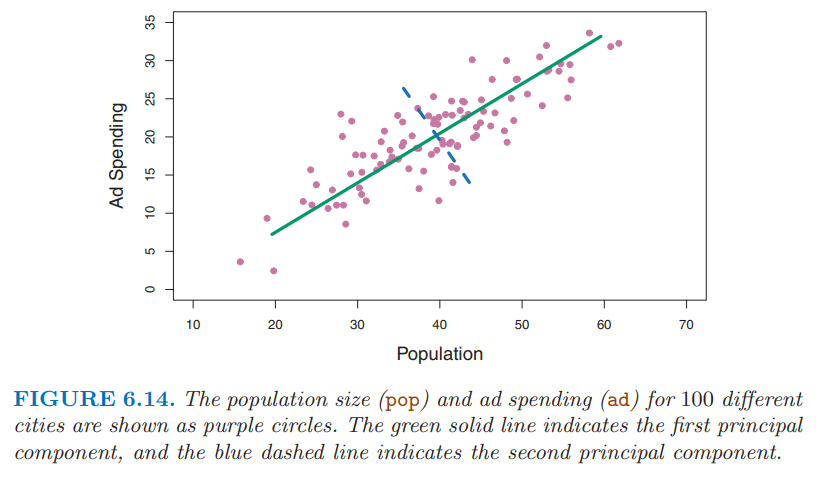
\includegraphics[scale=0.8]{images/first princ comp.png}
\end{center}
Projecting a point onto a line simply involves finding the location on the line which is closest to the point. The first principal component in the figure is given by the formula:
\begin{equation}
    Z_1 = 0.839 \times (pop - \overline{pop}) + 0.544 \times (ad - \overline{ad})
    \label{example}
\end{equation}
Here $\phi_{11} = 0.839$ and $\phi_{21} = 0.544$ are the principal component loadings, which define the direction referred to above. In \ref{example}, $\overline{pop}$ indicates the mean of all $pop$ values in this data set, and $\overline{ad}$ indicates the mean of all advertising spending. The idea is that out of every possible linear combination of $pop$ and $ad$ such that $\phi_{11}^2 + \phi_{21}^2 = 1$, this particular linear combination
yields the highest variance: i.e. this is the linear combination for which $Var(\phi_{11} \times (pop - \overline{pop}) + \phi_{21} \times (ad - \overline{ad}))$ is maximized.

\subsection{Further principal components}
After the first principal component $Z_1$ of the features has been determined, we can find the second principal component $Z_2$. The second principal component is the linear combination of $X_1,...,X_p$ that has maximal variance out of all linear combinations that are \textit{uncorrelated} with $Z_1$. The second principal component scores $z_{12}, z_{22},...,z_{n2}$ take the form
\[z_{i2} = \phi_{12} x_{i1} + \phi_{22}x_{i2} + ... + \phi_{p2} x_{ip}\]
where $\phi_2$ is the second principal component loading vector.  It turns out that constraining $Z_2$ to be uncorrelated with $Z_1$ is equivalent to constraining the direction $\phi_2$ to be orthogonal (perpendicular) to the direction $\phi_1$, and so on.\\\\
Once we have computed the principal components, we can plot them
against each other in order to produce low-dimensional views of the data. For instance, we can plot the score vector $Z_1$ against $Z_2$, $Z_1$ against $Z_3$,
$Z_2$ against $Z_3$, and so forth.\\\\
We illustrate the use of PCA on the \textbf{USArrests} data set. For each of the
50 states in the United States, the data set contains the number of arrests
per 100,000 residents for each of three crimes: \textbf{Assault}, \textbf{Murder}, and \textbf{Rape}. We also record \textbf{UrbanPop} (the percent of the population in each state living in urban areas). The principal component score vectors have length $n = 50$, and the principal component loading vectors have length $p = 4$. PCA was performed after standardizing each variable to have mean zero and standard deviation one.
\begin{center}
    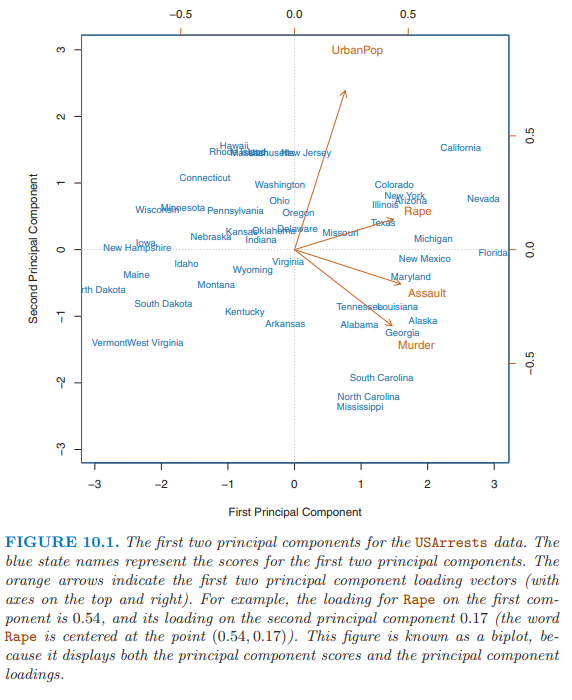
\includegraphics[]{images/biplot.png}
\end{center}
The figure above plots the first two principal components of these data. The figure represents both the principal component scores and the loading vectors in a single biplot display. The loadings are also given in the table below: 
\begin{center}
    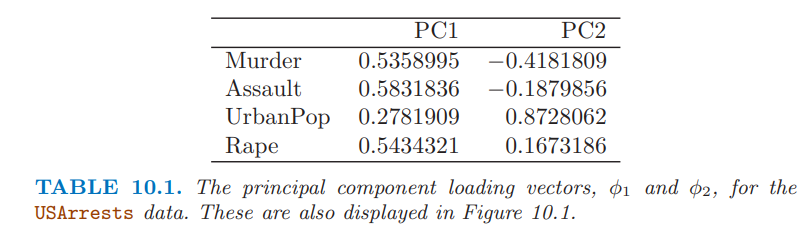
\includegraphics[scale=0.6]{images/table.png}
\end{center}
From the figure we see that the first loading vector places approximately
equal weight on \textbf{Assault}, \textbf{Murder}, and \textbf{Rape}, with much less weight on \textbf{UrbanPop}. Hence this component roughly corresponds to a measure of overall rates of serious crimes. The second loading vector places most of its weight
on \textbf{UrbanPop} and much less weight on the other three features. Hence, this
component roughly corresponds to the level of urbanization of the state. Overall, we see that the crime-related variables (\textbf{Murder}, \textbf{Assault}, and \textbf{Rape}) are located close to each other, and that the \textbf{UrbanPop} variable is far from the other three. This indicates that the crime-related variables are correlated with each other—states with high murder rates tend to have high
assault and rape rates—and that the \textbf{UrbanPop} variable is less correlated with the other three.\\\\
We can examine differences between the states via the two principal component score vectors shown in the figure. Our discussion of the loading vectors suggests that states with large positive scores on the first component, such as California, Nevada and Florida, have high crime rates, while states like North Dakota, with negative scores on the first component, have low crime rates. California also has a high score on the second component, indicating a high level of urbanization, while the opposite is true for states like Mississippi. States close to zero on both components, such as Indiana, have approximately average levels of both crime and urbanization.

\section{Another Interpretation of Principal Components}
The first two principal component loading vectors in a simulated three-dimensional data set are shown in the left-hand panel of the Figure below.
\begin{center}
    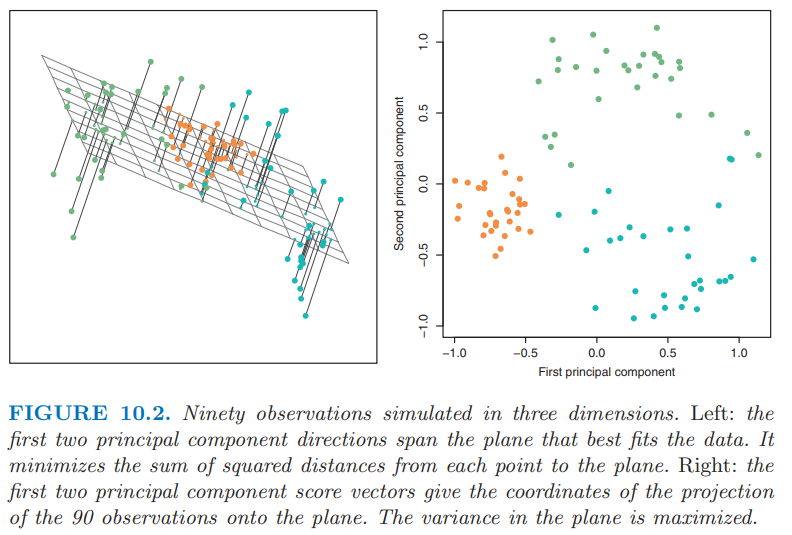
\includegraphics[scale=0.8]{images/3d pca.png}
\end{center}
Principal components provide low-dimensional linear surfaces that are closest to the observations. We expand upon that interpretation here. The first principal component loading vector has a very special property: it is the line in $p$-dimensional space that is closest to the n observations (using average squared Euclidean distance as a measure of closeness). The appeal of this interpretation is clear: we seek a single dimension of the data that lies as close as possible to all of the data points, since such a line will likely provide a good summary of the data.\\\\
The notion of principal components as the dimensions that are closest to the n observations extends beyond just the first principal component.  For instance, the first two principal components of a data set span the plane that is closest to the n observations, in terms of average squared Euclidean distance.

\section{Scaling the Variables}
We have already mentioned that before PCA is performed, the variables should be centered to have mean zero. Furthermore, the results obtained when we perform PCA will also depend on whether the variables have been individually scaled (each multiplied by a different constant).
\begin{center}
    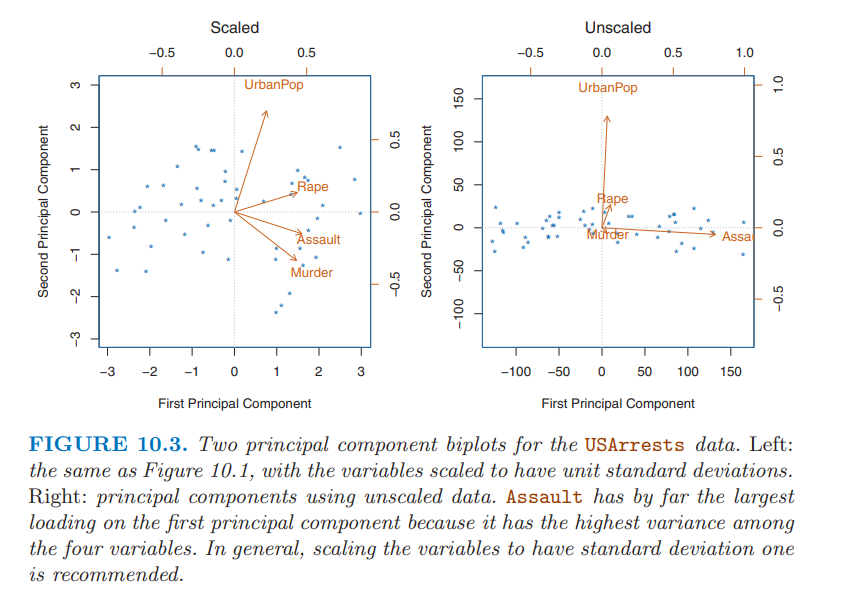
\includegraphics[scale=0.8]{images/scaled pca.png}
\end{center}
From the figure above, we see that scaling does indeed have a substantial effect on the results obtained. In these data, the variables are measured in different units; \textbf{Murder}, \textbf{Rape}, and \textbf{Assault} are reported as the number of occurrences per 100, 000 people, and \textbf{UrbanPop} is the percentage of the state’s population that lives in an urban area. These four variables have variance 18.97, 87.73, 6945.16, and 209.5, respectively. Consequently, if we perform PCA on the unscaled variables, then the first principal component loading vector will have a very large loading for \textbf{Assault}, since that variable has by far the highest variance.
\\\\
Because it is undesirable for the principal components obtained to depend on an arbitrary choice of scaling, we typically scale each variable to have standard deviation one before we perform PCA. In certain settings, however, the variables may be measured in the same units. In this case, we might not wish to scale the variables to have standard deviation one before performing PCA.

\section{The Proportion of Variance Explained}
In Figure 10.2, we performed PCA on a three-dimensional data set (lefthand panel) and projected the data onto the first two principal component loading vectors in order to obtain a two-dimensional view of the data  (i.e. the principal component score vectors; right-hand panel). We see that this two-dimensional representation of the three-dimensional data does successfully capture the major pattern in the data.\\\\
We can now ask a natural question: how much of the information in a given data set is lost by projecting the observations onto the first few principal components? That is, how much of the variance in the data is not contained in the first few principal components? More generally, we are interested in knowing the \textbf{proportion of variance explained} (PVE) by each principal component.\\\\
The total variance present in a data set (assuming that the variables have been centered to have mean zero) is defined as:
\[\sum_{j=1}^p Var(X_j) = \sum_{j=1}^p \frac{1}{n} \sum_{i=1}^n x_{ij}^2\]
and the variance explained by the $m$-th principal component is
\[\frac{1}{n}\sum_{i=1}^n z_{im}^2\]
Therefore, the PVE of the $m$-th principal component is given by:
\[\frac{\sum_{i=1}^n z_{im}^2}{\sum_{j=1}^p\sum_{i=1}^n x_{ij}^2}\]
In total, there are $min(n - 1, p)$ principal components, and their PVEs sum to one.

\section{Deciding How Many Principal Components to Use}
If we use principal components as a summary of our data, how many components are sufficient?  Unfortunately, there is no single (or simple!) answer to this question. We typically decide on the number of principal components required to visualize the data by examining a scree plot, such as the one shown in the left-hand panel of Figure 10.4.
\begin{center}
    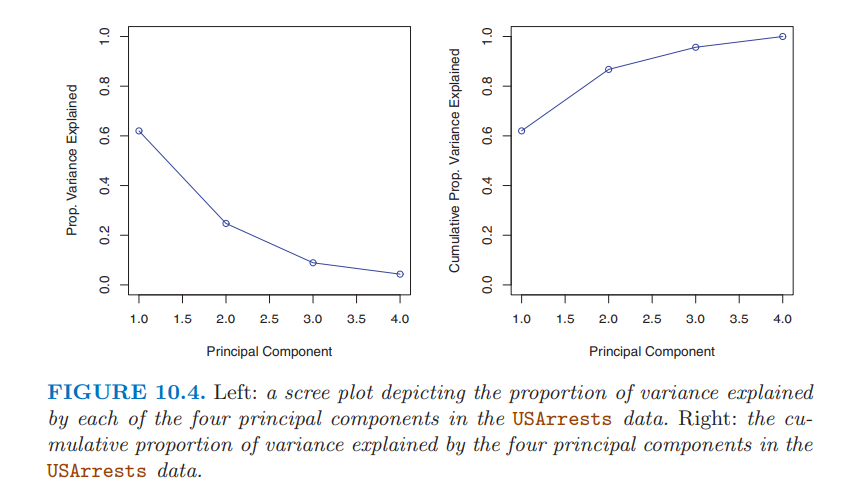
\includegraphics[scale=0.8]{images/scree plot.png}
\end{center}
